\documentclass[12pt,fleqn,answers]{exam}
\usepackage{pifont}
\usepackage{dingbat}
\usepackage{amssymb}
\usepackage{epsfig}
\usepackage{graphicx}
\usepackage[]{hyperref}
\usepackage{geometry}
\usepackage[intlimits]{amsmath}
\geometry{letterpaper, margin=0.75in}
\addpoints
\boxedpoints
\pointsinmargin
\pointname{pts}

\usepackage[activate={true,nocompatibility},final,tracking=true,kerning=true,factor=1100,stretch=10,shrink=10]{microtype}
\usepackage[american]{babel}
%\usepackage[T1]{fontenc}
\usepackage{fourier}
\usepackage{isomath}
\usepackage{upgreek,amsmath}
\usepackage{amssymb}

\newcommand{\dotprod}{\, {\scriptzcriptztyle
    \stackrel{\bullet}{{}}}\,}

\newcommand{\reals}{\mathbf{R}}
\newcommand{\lub}{\mathrm{lub}} 
\newcommand{\glb}{\mathrm{glb}} 
\newcommand{\complex}{\mathbf{C}}
\newcommand{\dom}{\mbox{dom}}
\newcommand{\cover}{{\mathcal C}}
\newcommand{\integers}{\mathbf{Z}}
\newcommand{\vi}{\, \mathbf{i}}
\newcommand{\vj}{\, \mathbf{j}}
\newcommand{\vk}{\, \mathbf{k}}
\newcommand{\bi}{\, \mathbf{i}}
\newcommand{\bj}{\, \mathbf{j}}
\newcommand{\bk}{\, \mathbf{k}}
\DeclareMathOperator{\Arg}{\mathrm{Arg}}
\DeclareMathOperator{\Ln}{\mathrm{Ln}}
\newcommand{\imag}{\, \mathrm{i}}
\newcommand{\range}{\mathrm{range}}
\newcommand{\ball}{\mathrm{ball}}
\newcommand{\LP}{\mathrm{LP}}

\newcommand{\signum}{\mathrm{sgn}}

\usepackage{graphicx}
\newcommand\AM{{\sc am}}
\newcommand\PM{{\sc pm}}
     
\newcommand{\quiz}{0}
\newcommand{\term}{Fall}
\newcommand{\due}{Friday 25 August  at 11:59 \PM}
\begin{document}
\large
\vspace{0.1in}
\noindent\makebox[3.0truein][l]{{\bf MATH 202}}
{\bf Name:} \hrulefill \\
\noindent \makebox[3.0truein][l]{\bf Calculus Practice IV, \term \/ \the\year}
%{\bf Row:}\hrulefill\
\vspace{0.1in}

\noindent Here is an opportunity for you to maintain your calculus skills
over the summer. If you complete these problems,
digitize your work, and submit your work to Canvas, I will send you my
solutions. If you need some help with these questions, 
email me with your questions (\href{mailto:willisb@unk.edu}{willisb@unk.edu})

Completing this work is optional, and it does not 
enter into your class grade in any way--this work is 
 not a bonus, extra credit, or anything like that.

\begin{questions}


\question The graph in Figure 1 shows the graph of a wild and 
crazy function (the red curve) whose domain is $[-4,4]$ that
we'll unimaginatively call $F$. Define a function $G$ by
\begin{equation*}
   G(x) = \int_{-4}^x F(s) \, \mathrm{d} s.
\end{equation*}

As best you can, draw a graph of $G$.

\begin{figure}[h]
\begin{center}
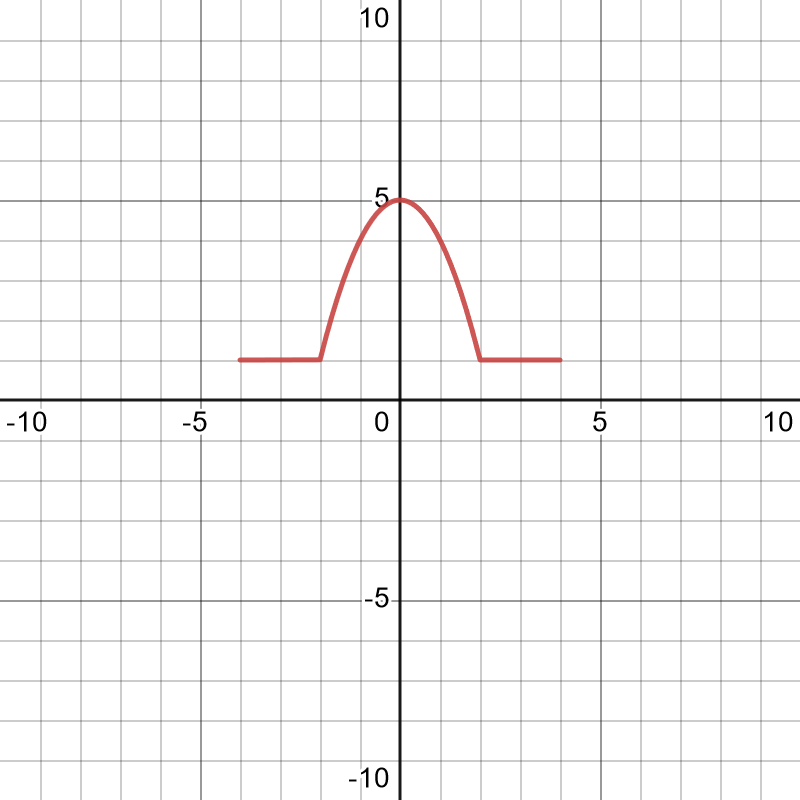
\includegraphics[scale=0.4]{desmos-graph(49).png}
\end{center}
\caption{Graph of some wild and crazy function.}
\end{figure}
\end{questions}

\begin{solution}

To start, let's review the properties of a function $G$ that is defined by
\begin{equation*}
    G(x) = \int_{a}^x F(s) \, \mathrm{d}s,
\end{equation*} 
where $F$ is integrable on an interval $[a,b]$. We have:

\begin{itemize}
\item $G(a)=0$
\item $G$ is continuous on $[a,b]$.
\item $G$ is differentiable everywhere that $F$ is continuous.
\item Wherever $F$ is continuous, we have $G^\prime(x) = F(x)$.
\end{itemize}
Specifically for our function $F$ given graphically in Figure 1, we 
conclude that (a) $G(-4) = 0$, (b) $G$ is continuous on $[-4,4]$  
  (c)$G^\prime(x) = F(x)$  on $[-4,4]$. Further, since 
 $F(x) > 0$, we see 
  that $G^\prime(x) > 0$. This means that $G$ is an increasing 
  function. The steepest part of the graph of $G$ is at $0$, where
  $G^\prime(0) = 5$.  Finally, the derivative of $G$ is constant on 
  the interval $[-4,-1]$, so $G$ is a linear function on this interval.
  The same is true on the interval $[1,4]$.

  Putting all this together, a graph of $G$ looks something like

  \vfill 
  \newpage 
    \begin{center}
    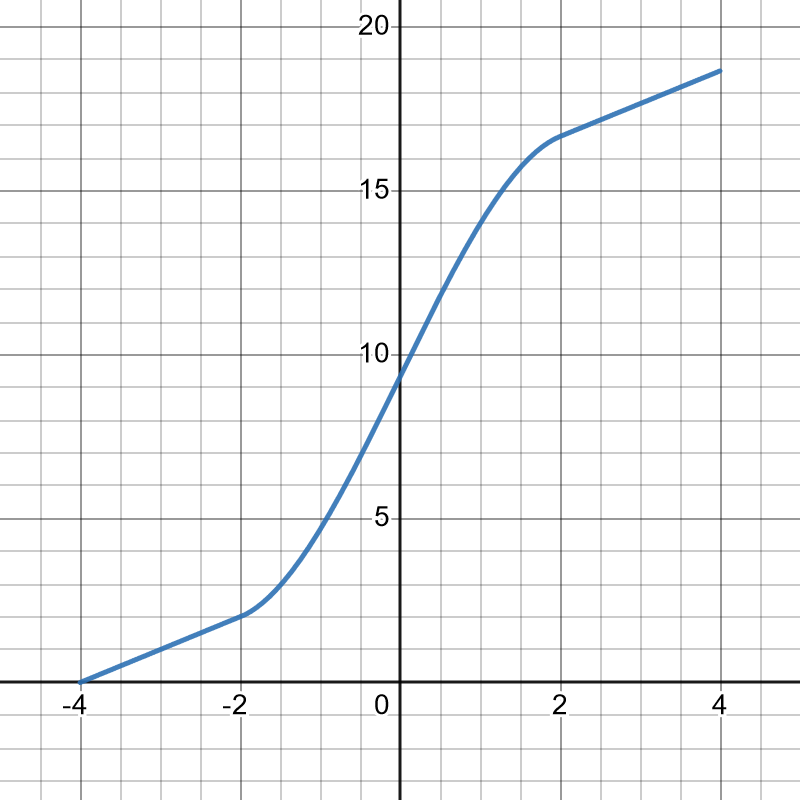
\includegraphics[scale=0.4]{desmos-graph(51).png}
  \end{center}

I know what you are thinking: Isn't the middle part of the graph 
a downward facing parabola surrounded by two shorter constant 
portions? Specifically, isn't the formula for $F$ something like
\begin{equation*}
    F(x) = \begin{cases} 1 & -4 \leq x \leq -2 \\
                         5-x^2 & -2 < x < 2 \\
                         1     & 2 \leq x \leq 4
    \end{cases}?
  \end{equation*}    
Sure, the graph of $F$ agrees with this formula. So we can find a 
formula for $F$ by integrating. For $-4 \leq x \leq -2$, we have
\begin{equation*}
  G(x) = \int_{-4}^x \, \mathrm{d} s = x+4.
\end{equation*}
And for $-2 < x < 2$, we have
\begin{equation*}
  G(x) = \int_{-4}^{-2} \, \mathrm{d} s + 
  \int_{-2}^{x} 5 - s^2 \, \mathrm{d} s =
    2 + -\frac{{{x}^{3}}}{3}+5 x+\frac{22}{3}
     = -\frac{{{x}^{3}}}{3}+5 x+\frac{28}{3}
\end{equation*}
And finally for $2 \leq x \leq 4$, we have
\begin{equation*}
G(x) = \int_{-4}^{-2} \, \mathrm{d} s + 
\int_{-2}^{2} 5 - s^2 \, \mathrm{d} s 
+ \int_2^x  \, \mathrm{d} s = 
x+\frac{44}{3}.
\end{equation*}
\end{solution}
Putting this together, a formula for $G$ is
\begin{equation*}
  G(x) = \begin{cases} x+4 & -4 \leq x \leq -2 \\
    -\frac{{{x}^{3}}}{3}+5 x+\frac{28}{3} & -2 < x < 2 \\
    x+\frac{44}{3}     & 2 \leq x \leq 4
  \end{cases}.
\end{equation*}   
Another way to do this is to find the antiderivative of each
case of the split rule and then to adjust the arbitrary constant
for each case to make the function $G$ continuous at -2 and 2. 
This calculation looks like this
\begin{equation*}
    G(x) = \begin{cases} x + c_1  & -4 \leq x \leq -2 \\
                         5x - \frac{1}{3} x^3 + c_2 & -2 < x < 2 \\
                         x+ c_3    & 2 \leq x \leq 4
    \end{cases}.
  \end{equation*}  
To make $G(-4)=0$, we need $-4 + c_1 = 0$; to make $G$ continuous 
at $-2$, we need $c_2 -\frac{22}{3}=c_1-2$; and to make $G$ continuous at 2, 
we need $c_2+\frac{22}{3}=c_3+2$. These are linear equations for $c_1,c_2$, and $c_3$.
Solving them, we get $c_1 = 4, c_2 = \frac{28}{3}$ and $c_3=\frac{44}{3}$.
    
And for something to ponder: a formula for $G$ that is not 
explicitly a split rule is 
\begin{equation*}  
G(x) = \frac{\signum\left( x-2\right)  {{\left( x-2\right) }^{2}}\, \left( x+4\right)  \signum\left( x+2\right) +32 \signum\left( x+2\right) -{{x}^{3}}+18 x+40}{6},
\end{equation*}
where the sign function $\signum$ is defined by
\begin{equation*}
   \signum(x) = \begin{cases} -1 & x < 0 \\ 0 & x=0 \\ 1 & x>0 \end{cases}.
\end{equation*}
Possibly this all-in-one formula has its appeal, but I'd say that 
the split rule formula is simpler for me to understand.
\end{document}